%*----------- SLIDE -------------------------------------------------------------
\begin{frame}[c]{Método BiLi}
    %\transboxin[duration=1,direction=30]
    \begin{figure}
        \centering
        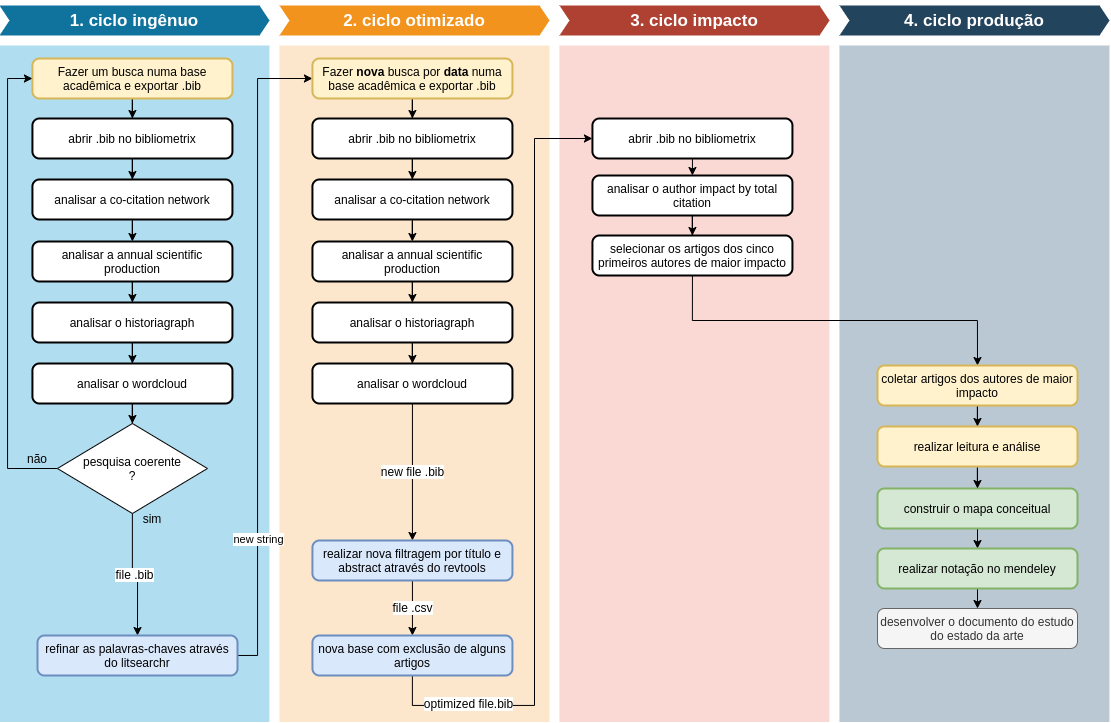
\includegraphics[width=0.7\textwidth]{bili-fluxograma.png}
    \end{figure}
%*----------- notes
    \note[item]{Notes can help you to remember important information. Turn on the notes option.}
\end{frame}
%-

%*----------- SLIDE -------------------------------------------------------------
\begin{frame}[c]{Mapa de Palavras}
    \framesubtitle{Ciclo Ingênuo X Ciclo Otimizado}
    %\transboxin[duration=1,direction=30]
    \begin{figure}
        \centering
        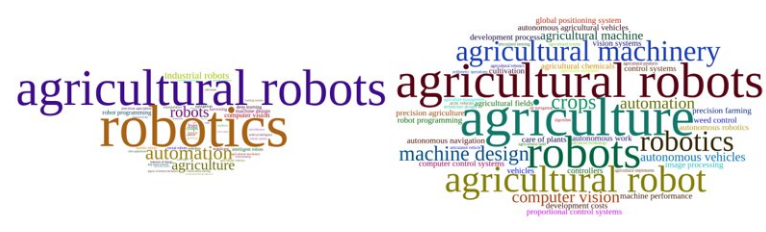
\includegraphics[width=1\textwidth]{bili-wordclould.png}
    \end{figure}
%*----------- notes
    \note[item]{Notes can help you to remember important information. Turn on the notes option.}
\end{frame}
%-

%*----------- SLIDE -------------------------------------------------------------
\begin{frame}[c]{Evolução Temática}
    %\transboxin[duration=1,direction=30]
    O tema de pesquisa apresentou \textbf{crescimento anual} de produção científica de \textbf{10,76\%} (2016 - 2021)\\
    \begin{figure}
        \centering
        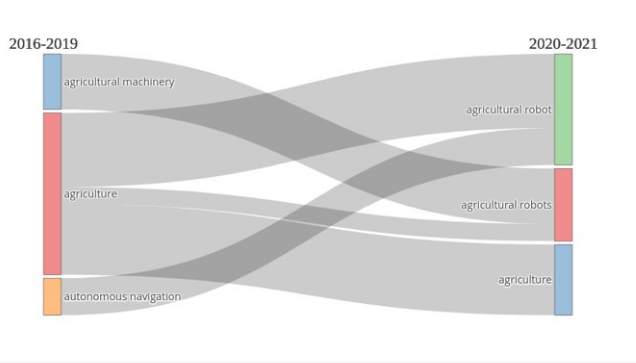
\includegraphics[width=0.65\textwidth]{bili-thematic-evolution.png}
    \end{figure}
%*----------- notes
    \note[item]{Notes can help you to remember important information. Turn on the notes option.}
\end{frame}
%-

%*----------- SLIDE -------------------------------------------------------------
\begin{frame}[c]{Referencial Teórico}
    \begin{table}[]
        \begin{tabular}{cc}
        \hline
        TEMA & AUTOR(ES) \\ \hline
        a    & 1          \\ \hline
        b    & 2         \\ \hline
        c    & 3         \\ \hline
        Sistema autônomo para plantio e colheita   & 4        
        \end{tabular}
        \end{table}
%*----------- notes
    \note[item]{Notes can help you to remember important information. Turn on the notes option.}
\end{frame}
%-